\chapter{Background}\label{chapter:background}
In this chapter, we formalize the reinforcement learning problem and discuss briefly various class of reinforcement learning algorithms.

\section{Markov Decision Process}
Markov Decision Process (MDP) provides a mathematical framework to formalize sequential decision making. MDP describes an agent interacting with a stochastic environment. The decision maker and learner are called the agent, everything else is referred to as the environment. The interaction between agent and environment happen continuously in discrete time steps. At each time step $t$, the agent selects action and environment respond to the action by presenting a new situation for the agent. \\

% \noindent
An MDP has following components:
\begin{itemize}
\item $\mathcal{S}$ is a finite set of environment states.
\item $\mathcal{A}$ is a finite set of actions available for agent at a state.
\item $p(s_{t+1}|s_t, a_t)$ is the transition probability distribution. It represents the probability that an action $a_t$ in state $s_t$ at time $t$ will lead to state $s_{t+1}$ at time $t+1$.
\item $r(s_t, a_t, s_{t+1}) \in \mathbb{R}$ is the reward received by the agent after taking an action $a_t$ at state $s_t$ and reaching at state $s_{t+1}$.
\item $\gamma \in [0,1]$ is the discount factor, which determines present value of future rewards.
\end{itemize}

\begin{figure}[!htb]
    \centering
    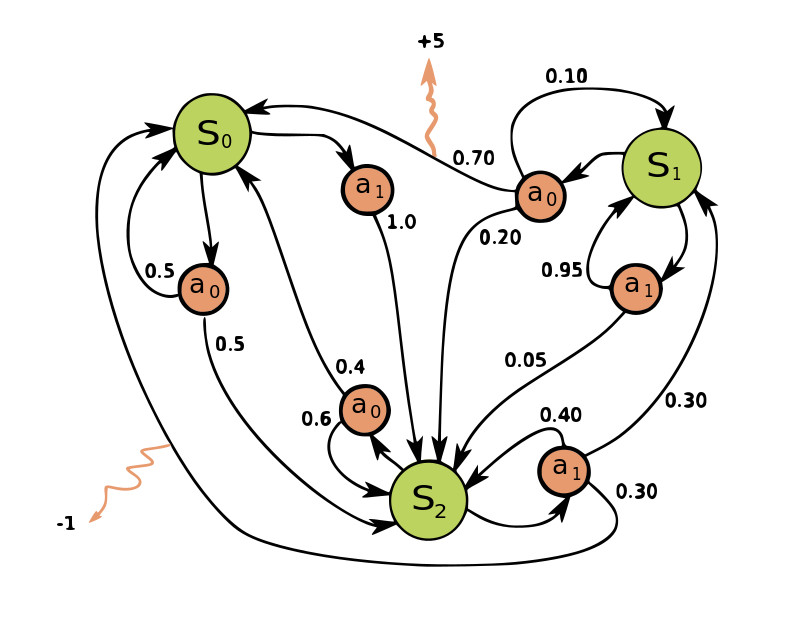
\includegraphics[width=.8\linewidth]{figures/02/mdp.jpg}
    \caption{An example of MDP with three states and two actions. The orange arrows represent rewards emitted by environment to agent. The labels on edges are transition probabilities. Source: Wikipedia.}
    \label{fig:02_mdp}
\end{figure}

Sometimes the initial state distribution $\mu(s)$ is also provided, which is used to sample the initial state $s_0$.

The core problem of MDP is to find a \textit{policy} for the agent, a function $\pi(s)$ which maps a state $s$ to action chosen by the agent. The policy $\pi$ should be such that it maximizes the cumulative reward received by the agent over multiple interactions with the environment. In stochastic policies, $\pi$ is a conditional distribution $\pi(a|s)$ from which actions are sampled. The state transitions of an MDP satisfy the \textit{Markov property}, i.e. the transition probabilities are independent of previous states and only depend on current state $s_t$. A simple MDP with three states and two actions is illustrated in Figure \ref{fig:02_mdp}.


\section{Reinforcement Learning Problem}
Reinforcement learning can be studied mathematically as an MDP. An RL problem can be episodic or continuous depending on the task at hand. In episodic RL problems, the agent reaches a terminal state after a finite number of steps; one such finite interaction is termed as an \textit{episode}. Whereas in continuous RL problems, the agent interacts continuously with the environment and there is no terminal state. The notion of cumulative reward breaks in case of continuous RL problem as it can have infinite steps.     So, instead of cumulative reward, discounted return is maximized and is defined at time step $t$ with discount factor $\gamma$ as 

\begin{equation}\label{eq:discreward}
R_t = \sum_{i=t}^\infty \gamma^{i-t}r(s_i, a_i, s_{i+1}).
\end{equation}

The states $s_i$ are generated by sampling actions from some policy $\pi(a_i|s_i)$. The discount factor $\gamma$ is needed to weight the importance of future rewards. For $\gamma=0$, the agent is only concerned with maximizing immediate reward, as $\gamma$ increases the agent becomes far-sighted and acts to maximize future rewards as well. Usually, $\gamma \in [0.9, 0.99]$ is most commonly used. Discount return is also valid for episodic RL problems as those can be reduced to continuous RL problems by adding a self-loop at terminal states with transition probability 1. 

The discounted reward can be recursively written as 

\begin{equation}\label{eq:recdiscreward}
R_t = r(s_t, a_t, s_{t+1}) + \gamma R_{t+1}.
\end{equation}

Thus, the goal of reinforcement learning algorithms is to find a policy that maximizes the expected future reward.

\section{Value Functions}
A value function represents how good it is to be in a particular state. Value functions are important as they provide a framework to optimize agent policies and a lot of reinforcement learning algorithms use value functions in some form. 

\subsection{Definition}

\textbf{Value function} is formally defined in terms of expected future rewards at a state. Since future rewards depend on the policy of the agent, therefore the value functions are defined with respect to policies. A value function can be dependent on state only or on state-action pair. A state dependent value function $V_\pi(s_t)$ is called state-value function and is defined as expected future reward starting from $s_t$ and then following the policy $\pi(a_t|s_t)$. It can be formally written as

\begin{equation}
\label{eq:vfunction}
V_\pi(s_t) = \mathbb{E}_\pi[R_t|s_t] = \mathbb{E}_\pi\left[\sum_{i=t}^\infty \gamma^{i-t}r(s_i, a_i, s_{i+1})|s_t\right],
\end{equation}

where $\mathbb{E}_\pi[.]$ denotes the expected value of a random variable given that the agent follows policy $\pi$, and $t$ is any time step.

The state-action value function is called Q-function and is denoted by $Q_\pi(s_t,a_t)$. The Q-function is defined as the expected return starting from $s$, taking an action $a$ and then following the policy $\pi(a_t|s_t)$. It can be formally written as

\begin{equation}
\label{eq:qfunction}
Q_\pi(s_t,a_t) = \mathbb{E}_\pi[R_t|s_t,a_t] = \mathbb{E}_\pi\left[\sum_{i=t}^\infty \gamma^{i-t}r(s_i, a_i, s_{i+1})|s_t, a_t\right].
\end{equation}

The value function satisfies a recursive relation which follows from Eqn. \ref{eq:recdiscreward}, \ref{eq:vfunction} and \ref{eq:qfunction}, called Bellman equation. For any policy $\pi$, the following always hold for value functions

\begin{equation}\label{eq:bellman_v}
V_\pi(s_t) = \mathbb{E}_{s_{t+1}\sim p, a_t \sim \pi}[r(s_t,a_t,s_{t+1}) + \gamma V_\pi(s_{t+1})],
\end{equation}

\begin{equation}\label{eq:bellman_q}
Q_\pi(s_t,a_t) = \mathbb{E}_{s_{t+1}\sim p}[r(s_t,a_t,s_{t+1}) + \gamma\mathbb{E}_{a_{t+1}\sim\pi}[Q_\pi(s_{t+1},a_{t+1})]].
\end{equation}

\subsection{Optimal Value Functions}
A policy $\pi^1$ is better than $\pi^2$ if $V_{\pi^1}(s) \geq V_{\pi^2}(s) $ for all possible states $s$. There exist policies which are always better than all other policies, called optimal policies. The optimal policy $\pi^*$ for a given reinforcement learning task can be found by finding the optimal value function:

\begin{equation}\label{eq:bellmanv_opt}
V^*(s) = \max_\pi V_\pi(s),
\end{equation}

\begin{equation}\label{eq:bellmanq_opt}
Q^*(s,a) = \max_\pi Q_\pi(s,a).
\end{equation}

Optimal value function gives the best possible total reward. Since $Q^*$ represents the optimal value function, the best value at step $t+1$ is just the action which has highest Q-value. So, the Bellman equation (see Eqn. \ref{eq:qfunction}) for the optimal Q-value function $Q^*$ can be written without referencing any other policy $\pi$. The optimal policy $\pi^*$ for $Q^*$ is therefore the greedy policy $\max_{a\in A} Q^*_{\pi^*}(s, a)$. The Bellman equation for optimal Q-value, known as Bellman optimality condition can be written as

\begin{equation}\label{eq:bellman_v}
Q^*_\pi(s_t, a_t) = \mathbb{E}_{s_{t+1}\sim p}[r(s_t,a_t,s_{t+1}) + \gamma \max_{a^\prime \in A} Q^*_{\pi^*}(s_{t+1}, a^\prime)].
\end{equation}

A similar optimality condition holds for state-value function $V^*$ as well.

% add more information about 
\newpage
\section{Policy Optimization}

As discussed in the last section, the goal of a reinforcement learning algorithm is to find a policy that maximizes the expected future rewards. There are various approaches to find such a policy and could be broadly classified in following two types:

\subsection{Value Iteration}
Value iteration algorithms search for an optimal value function. The value function is initialized randomly in the beginning and then improved iteratively until optimal value function is found. The value function is improved at each iteration using the Bellman equation (see Eqn.\ref{eq:bellman_q}). Once optimal value function has been found, the optimal policy can be extracted from value function by choosing a greedy actions at each state. 

\subsection{Policy Iteration}
Policy iteration algorithms find the optimal policy by alternating between policy evaluation and policy improvement. The agent starts with a random policy, finds the value function for the policy (policy evaluation), then improves the policy based on previous value function. The value function is found using Eqn. \ref{eq:qfunction}. In many problems, policy iteration converges faster than value iteration because policy function is easier to represent than the value function. For example, in case of Atari games, it is easier to represent a policy which predicts the next action at an image frame rather than representing a function which predicts the expected reward for all actions at that frame.

\section{Function Approximation}
In real-world problems, finding an optimal policy is computationally impossible as the problem state space increases exponentially with increase in state dimensionality. In such cases, only an approximation to the optimal policy can be found. There are many choices for function approximators such as decision trees, nearest neighbor, neural networks. Out of these, neural networks had a lot of success recently in a variety of reinforcement learning problems and are commonly used nowadays.

Depending on which part of the problem is modeled with neural networks, there exist a variety of algorithms. The different categories of model-free algorithms are listed below.

\begin{itemize}
\item \textbf{Value Based Methods} learn a value function and have an implicit greedy policy. The value function is represented by a neural network as $Q(s,a|\theta^Q)$, where $\theta^Q$ are network parameters. The value function network can either take state $s$ as input and output Q-values for all $(s,a)$ pairs or take $(s,a)$ as input and output a single Q-value. DQN \cite{01_dqn} is a value based algorithm which learns Q-values for all $(s,a)$ pairs.

\item \textbf{Policy Based Methods} learn the policy directly and no value function is used. The policy is represented by a neural network as $\pi(a|s,\theta^\pi)$, where $\theta^\pi$ are network parameters. Alpha Go \cite{Silver_2016} uses a policy based method which trains a policy network with Monte-Carlo tree search. 

\item \textbf{Actor-Critic Methods} are a mix of both value-based and policy-based algorithms. These have two networks, an actor network which represents the policy and a critic network which represents the value function. Sometimes actor and critic share some part of the network. The critic network is used to estimate the policy gradients for optimizing the policy network. Actor-critic methods are more common in continuous action space problems. A3C \cite{a3c} uses an actor-critic architecture, where multiple actor-critic networks are used for asynchronous training.

\end{itemize}

\section{Model-based and Model-free Reinforcement Learning}
\textbf{Model based reinforcement learning} algorithms build a model of the environment dynamics. The model contains the knowledge about the task at hand, such as transition probabilities and different possible immediate outcomes. These algorithms usually roll-out the entire trajectory by taking actions using the environment model and estimate the total reward for each action. The action with the highest total reward is then chosen. \cite{Nagabandi2017NeuralND}, SVG \cite{svg}, NAF \cite{gu2016} are some recently proposed model-based algorithms which use neural networks to the model environment dynamics.
\linebreak

\noindent
\textbf{Model-free reinforcement learning} algorithms, on the other hand, are based on estimating the expected returns at any state by learning a value function or learning a policy which maximizes expected returns. Model-free algorithms are easier to use but require a lot of trial and error to get a good estimate of the value function or the policy. DQN \cite{01_dqn}, DDPG \cite{ddpg}, A3C \cite{a3c} and TRPO \cite{schulman2015trust} are some recent model-free algorithms which have shown to perform well on variety of Atari games and robotic simulation tasks.

\section{On-policy and off-policy Algorithms}
A reinforcement learning algorithm can have two policies during training. One is used to generate the experience and explore the environment, while the second is the target optimal policy which is being learned by the agent. Depending on whether these policies are same or different it gives rise to two different class of algorithms. 

\textbf{On-policy algorithms} optimize the same policy which is used by the agent to explore the environment. SARSA \cite{sutton1998reinforcement} is an on-policy algorithm.

\textbf{Off-policy algorithms} use a different policy to explore the environment and optimize a different policy based on the generated experience. DQN is an off-policy learning algorithm.
% how to use neural networks in reinforcement learning.

\section{Training Techniques}
Using reinforcement learning directly with neural networks is often unstable and sample inefficient. The agent has to play millions of episodes to learn a policy and it is not guaranteed that the agent will learn a useful policy even after that. So, there are some common techniques to alleviate these problems. These techniques are described below.


\subsection{Experience Replay}
Experience replay \cite{Lin1992} is a technique in which the learning algorithm proceeds in two phases. First, it gathers experience and store transitions $(s_t, a_t, s_{t+1}, r_t)$ at each time step $t$ in a replay memory. In the second step, the algorithm randomly samples batches from the replay memory and applies the Bellman optimality equation (see Eqn. \ref{eq:bellmanq_opt}) to update the target Q-network. Experience replay has following advantages:

\begin{itemize}
\item It efficiently uses the agent's past experience by learning through it multiple times. This is important because generating experience in real-world is costly. Value function learning with neural networks does not converge quickly, so it is better to use multiple passes of same experience to train the network.
\item Most gradient-based algorithms assume data to be independent identically distributed (i.i.d.) which is achieved by randomly sampling from replay buffer. This leads to better convergence behavior.
\item Neural networks does not handle training with sequential data very well, which leads to \textit{catastrophic forgetting} \cite{French1999CatastrophicFI}. Catastrophic forgetting is common in RL problems because when new data is introduced (from experience with the environment), new updates to the network overwrite the previously acquired behaviour. Sampling old experience from the replay memory reduces this problem.
\end{itemize}

\subsection{Soft Target Updates}
Training neural networks can be unstable with reinforcement learning algorithms on many environments. This could be because the same network that is being optimized is also used for calculation of the target term in the loss function. This often leads to divergent behaviour \cite{ddpg} \cite{01_dqn}. 

The problem is solved by maintaining a target network in addition to a local network (the network being optimized directly). The target network is used for calculation of the target term in the loss function and the local network parameters are updated using this loss. In the beginning of training, the target network starts with the same parameters as the local network. During training, the parameters of the target network ($\theta^\prime$) are then slowly updated from the local network parameters ($\theta$). The update equation for target network parameters is given by 

\begin{equation}
\theta^\prime = (1-\tau)\theta^\prime + \tau \theta,
\end{equation}

where $\tau$ is usually $\ll$ 1.


% There is currently a wide adoption of deep neural networks for reinforcement learning. 
% Deep Q Networks (DQN) \cite{mnih2015humanlevel} directly learn the action-value function with a deep neural network. Although this method can handle very high dimensional inputs, such as images, it can only deal well with discrete and low dimensional action spaces. 
% Guided Policy Search \cite{levine2013guided} can exploit high and low dimensional state descriptions by concatenating the low dimensional state to a fully connected layer inside the network.

% Recent methods for continuous control problems come in two flavours, \textit{vanilla policy gradient methods} which directly optimize the policy and \textit{actor-critic methods} which also approximate state-value function in addition to policy optimization. Trust Region Policy Optimization (TRPO) \cite{schulman2015trust} and Proximal Policy Optimization Algorithms \cite{SchulmanWDRK17} can be used as vanilla policy gradient as well as actor-critic methods. Whereas, Deep Deterministic Policy Gradient (DDPG) \cite{ddpg} and Asynchronous Advantage Actor Critic (A3C) \cite{a3c} use actor-critic architectures, where state-action function is learned to calculate policy gradients.

% Stochastic Value Gradients (SVG) \cite{svg}, Generalized Advantage Estimation (GAE) \cite{schulman2015trust}, A3C, TRPO all use \textit{stochastic policy gradients} and predict action probability distribution parameters. The action values are then sampled from the predicted distribution. A parametrized normal distribution is most commonly used as action distribution. This means that this formulation models a kind of action noise instead of the true action distribution. For example, a distribution with two modes cannot be modeled with a Gaussian.

% DDPG \cite{ddpg} which extends DPG \cite{silver2014deterministic} uses \textit{deterministic policy gradients} and achieves stability when using neural networks to learn the actor-critic functions. The limitation of DDPG is that it always gives a point estimate which may not be desired in stochastic action problems.

% % Stochastic policies have been used by \cite{wawrzynski2009real} and \cite{wawrzynski2013autonomous} to train a stochastic agent using replay buffers with an actor-critic algorithm. Further, TRPO \cite{schulman2015trust} directly learns a stochastic policy by containing the updates to the policy, so to carefully avoid performance drops during learning. 

% \cite{Lazaric2007} estimate stochastic action values using a sequential Monte Carlo method (SMC). SMC has actor and critic models where the actor is represented by Monte Carlo sampling weights instead of a general function approximator like a neural network. SMC learning works well in small state space problems, but cannot be extended directly to high dimensional non-linear action space problems.

% Similar to our idea of predicting multiple instead of one output, but originating from the domain of supervised learning, is Multiple Hypothesis Prediction \cite{rupprecht2017iccv}, which in turn is closely related to Multiple Choice Learning \cite{lee2016stochastic} and \cite{lee2017confident}. In this line of work, the model is trained to predict multiple possible answers for the given task. Specific care has to be taken since often in supervised datasets not all possible outcomes are labeled, this leading to loss functions that contain an $\argmin$-like term and, as such, are hard to differentiate.

